\documentclass[11pt]{article}
\usepackage{graphicx}
% Margins
\topmargin=-0.45in
\evensidemargin=0in
\oddsidemargin=0in
\textwidth=6.5in
\textheight=9.0in
\headsep=0.25in

\title{Description of Ising Computation Project}
\author{Gustaf Lundborg}
\date{\today}

\begin{document}
\maketitle
\pagebreak

% Optional TOC
% \tableofcontents
% \pagebreak

%--Paper--

\section{Purpose}
There has lately been a big interest in using so called Ising Systems for problem solving. This work includes the work on some so called Quantum Computers, algorithmic research on using the Ising Model for solving NP-complete problems, and also developing silicon implementations of Ising Systems.

The advantages of using Ising Models in these cases range from speed and energy conservation to being a central feature of the work.

Almost all this work has been focused on using the Ising Model as a means of doing optimizations. Here I am trying to take this a step further by using an Ising System to perform a Monte Carlo simulation.

This simulation is performed on a theoretical Ising circuit. Ising Models are usually solved using Monte Carlo simulations, what I am doing is simply reversing that process. However to get a result from my theoretical Ising circuit, this needs to be solved somehow. The most straightforward way is using a Monte Carlo simulation. So, in effect, I will do several Monte Carlo simulations to perform a single Monte Carlo simulation. While this may seem backwards, the purpose of this work is not to present a new algorithm for doing such simulations, but a proof of concept for new exploration. As such, the Ising Circuit should be regarded as a black box where the equilibrium state of the system provides a piece of the simulation.

For the sake of completeness, one should mention that the part of the simulation that the Ising circuit performs can be regarded as an optimization. However, this problem is so specific that there is no extra insight gained from calling it an optimization.

\section{Simulation Setup}
\subsection{General Idea}
The idea is do a Monte Carlo simulation to solve some real problem using an Ising Circuit. Monte Carlo simulations are often used in cases where the probability distribution of the solution space is not known. One class of such methods are called Markov Chain Monte Carlo simulations. Where the desired distribution is constructed step wise using some predefined rules.

The idea here is to do this using an Ising Circuit. The equilibrium output of the circuit will be random solution that is in the correct solution space and therefore can be used directly in a probability calculation. To achieve this the Ising Circuit needs to be setup to reflect the desired distribution. This can be done directly analytically for small systems. For larger systems the circuit needs to be trained. Once the circuit has been setup correctly, it can be used to generate sample solutions for the simulation. The circuit is initiated with random input and let to relax to equilibrium. The equilibrium state will represent a random sample for the simulation.

The system used here to try this is the problem of the self avoiding random walk (SAWs). One way to study SAWs numerically is to do a random walk on a grid and generate as many walks as possible. When a large enough number of sample walks have been generated, several statistical properties of the walk can be calculated. E.g. the root-mean-square (RMS) distance. No points in the grid can ever intersect or the walk is not a SAW. So, when doing numerical simulations, one of the simplest approaches is to generate many random walks and only keep those that fulfill the SAW criteria of non-intersection.
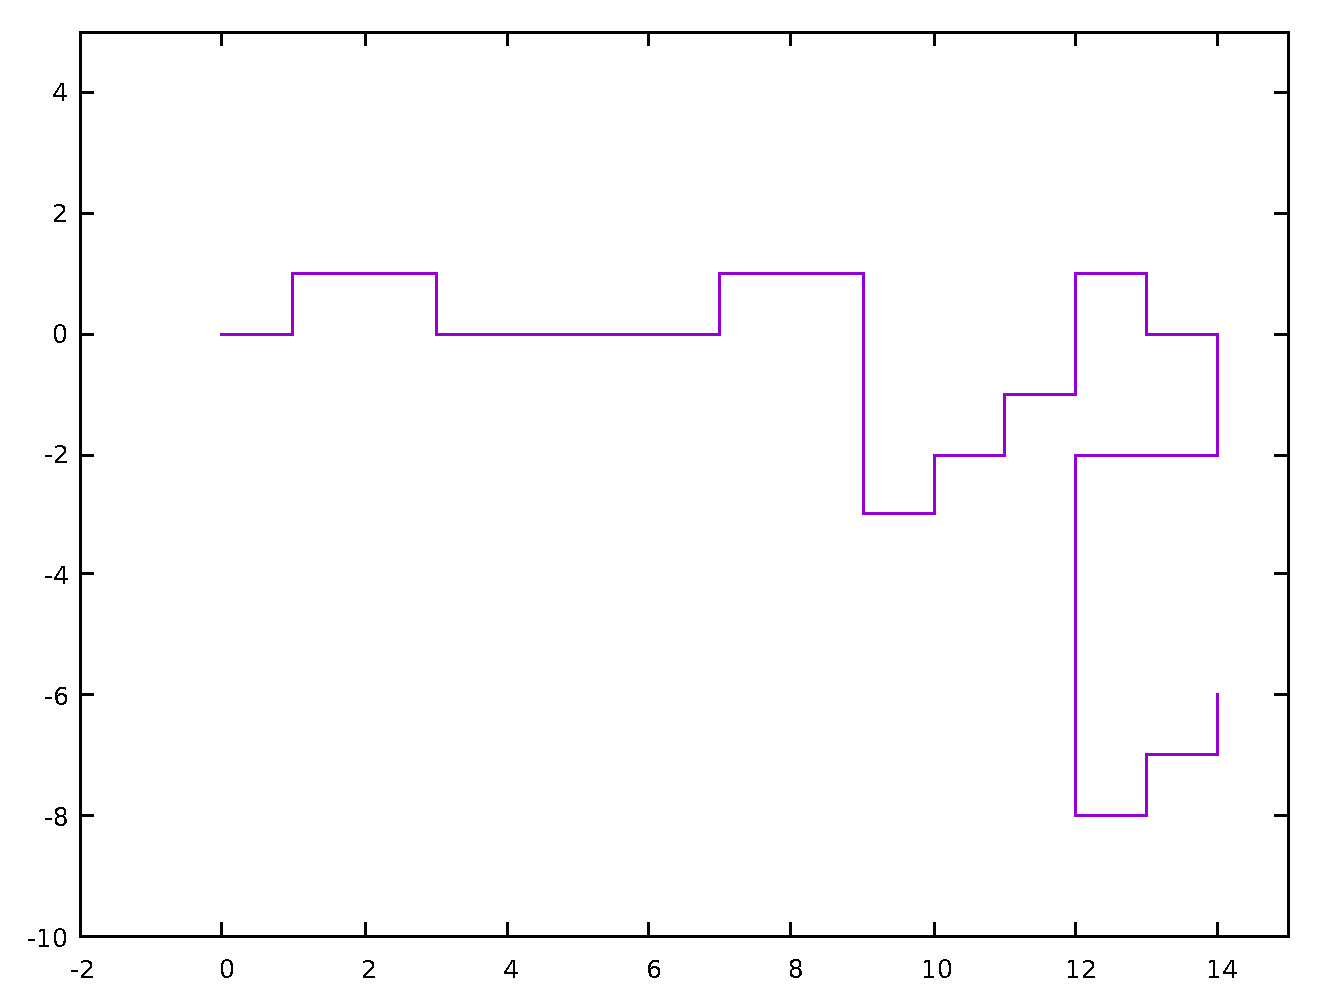
\includegraphics[scale=0.25]{images/saw_example.pdf}
\subsection{Ising Model}
\subsection{Self Avoiding Random Walk}
\subsection{Simulation outline}
\begin{itemize}
\item Generate many Random walks. Make sure they are NOT self avoiding and that they are unique.
\item Use random walks to train Ising Model connection matrix, by translating them to spins and maximize Hamiltonian.
\item Use arbitrary random walk translated to spins as starting seed. Anneal with temperature profile using connection matrix.
\item Save all unique self-avoiding random walks. (using tree. Extend anneal program to do this. Figure out way to check that the walks are nicely distributed)
\end{itemize}

\subsection{Data Representation}
A self avoiding random walk on a 2D grid is to be simulated. All walks start from the origin and have specific number of steps. Each step can take one of four directions \textbf{UP}, \textbf{DOWN}, \textbf{EAST} (intuitively to the right),  or \textbf{WEST} (to the left).
\section{Case study - Polymer simulation}
\subsection{Reference simulations}


\section{Results}

%% \pagebreak
%% \section{Section 2}

%--/Paper--

\end{document}
